
\newcommand*{\myBoxBlack}[6]{
	% 1 : p_x  --  4 : w_x
	% 2 : p_y  --  5 : w_y
	% 3 : p_z  --  6 : w_z
	\draw[black, fill=white] (#1,-#2,-#3) -- ++(-#4,0,0) -- ++(0,-#5,0) -- ++(#4,0,0) -- cycle;
	\draw[black, fill=white] (#1,-#2,-#3) -- ++(0,0,-#6) -- ++(0,-#5,0) -- ++(0,0,#6) -- cycle;
	\draw[black, fill=white] (#1,-#2,-#3) -- ++(-#4,0,0) -- ++(0,0,-#6) -- ++(#4,0,0) -- cycle;
}

\newcommand*{\myBoxBlackUnfilled}[6]{
	\draw[black] (#1,-#2,-#3) -- ++(-#4,0,0) -- ++(0,-#5,0) -- ++(#4,0,0) -- cycle;
	\draw[black] (#1,-#2,-#3) -- ++(0,0,-#6) -- ++(0,-#5,0) -- ++(0,0,#6) -- cycle;
	\draw[black] (#1,-#2,-#3) -- ++(-#4,0,0) -- ++(0,0,-#6) -- ++(#4,0,0) -- cycle;
}

\newcommand*{\myBoxGrey}[6]{
	\draw[black!60, fill=black!25] (#1,-#2,-#3) -- ++(-#4,0,0) -- ++(0,-#5,0) -- ++(#4,0,0) -- cycle;
	\draw[black!60, fill=black!25] (#1,-#2,-#3) -- ++(0,0,-#6) -- ++(0,-#5,0) -- ++(0,0,#6) -- cycle;
	\draw[black!60, fill=black!25] (#1,-#2,-#3) -- ++(-#4,0,0) -- ++(0,0,-#6) -- ++(#4,0,0) -- cycle;
}

	%%%%%%%%%%%%%%%%%%%%%%%%%%%%%%%%%%%%%%%%%%%% 
	%%% Draw the main framework
	%%%  With 3 processing thingy
	%%%  And a RNN
	%%%%%%%%%%%%%%%%%%%%%%%%%%%%%%%%%%%%%%%%%%%% 


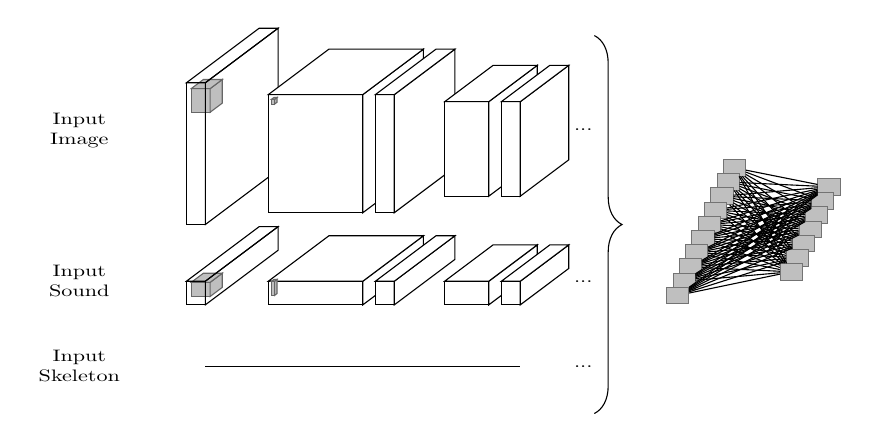
\begin{tikzpicture}[yscale=0.6, xscale=0.8, every node/.style={transform shape}]

	\node[text width=4em, text centered] (I-1) at (-2,-1) {Input Image};

	%%%%%%%%%%%%%%%%%%%%%%%%%%%%%%%%%%%%%%%%%%%% 
	%%% DRAW THE INPUT IMAGE
	%%%%%%%%%%%%%%%%%%%%%%%%%%%%%%%%%%%%%%%%%%%% 
	\myBoxGrey {0}{.2}{.2}{.3}{.5}{.5}
	\myBoxBlackUnfilled{0}{0}{0}{.3}{3}{3}

	%%% DRAW 1st ConvolutionLayer
	\myBoxBlack{2.5}{.25}{0}{1.5}{2.5}{2.5}
	\myBoxBlack{3}{.25}{0}{.3}{2.5}{2.5}
	\myBoxGrey{1.1}{.35}{0}{.05}{.1}{.1}

	%%% DRAW 2nd ConvolutionLayer
	\myBoxBlack{4.5}{.4}{0}{.7}{2}{2}
	\myBoxBlack{5}{.4}{0}{.3}{2}{2}

	%%%%%%%%%%%%%%%%%%%%%%%%%%%%%%%%%%%%%%%%%%%% 
	%%% draw split lines for Channels 
	% \foreach \channel in {1,...,15}{
	%     \draw[black,dashed] (2.5-\channel*.1,-.25,0) -- ++(0,-\cubey,0) ;
	%     \draw[black,dashed] (2.5-\channel*.1,-.25,0) -- ++(0,0,-\cubez) ;
	% }

	\node[text width=4em, text centered] (I-1) at (6,-1) {...};


	%%%%%%%%%%%%%%%%%%%%%%%%%%%%%%%%%%%%%%%%%%%% 
	%%% DRAW THE INPUT SOUND
	%%%%%%%%%%%%%%%%%%%%%%%%%%%%%%%%%%%%%%%%%%%% 
	\pgfmathsetmacro{\yPading}{4.2}
	\node[text width=4em, text centered] (I-1) at (-2,-\yPading) {Input Sound};
	\myBoxGrey {0}{.1-\yPading}{.2}{.3}{.3}{.5}
	\myBoxBlackUnfilled{0}{0-\yPading}{0}{.3}{.5}{3}
	\myBoxBlack{2.5}{0-\yPading}{0}{1.5}{.5}{2.5}
	\myBoxBlack{3}{0-\yPading}{0}{.3}{.5}{2.5}
	\myBoxGrey{1.1}{0-\yPading}{0}{.05}{.3}{.1}
	\myBoxBlack{4.5}{0-\yPading}{0}{.7}{.5}{2}
	\myBoxBlack{5}{0-\yPading}{0}{.3}{.5}{2}
	\node[text width=4em, text centered] (I-1) at (6,-\yPading) {...};

	%%%%%%%%%%%%%%%%%%%%%%%%%%%%%%%%%%%%%%%%%%%% 
	%%% DRAW THE INPUT SKELETON
	%%%%%%%%%%%%%%%%%%%%%%%%%%%%%%%%%%%%%%%%%%%% 
	\pgfmathsetmacro{\yPading}{6}
	\node[text width=4em, text centered] (I-1) at (-2,-\yPading) {Input Skeleton};
	\draw (0,-\yPading) -- (5,-\yPading);
	\node[text width=4em, text centered] (I-1) at (6,-\yPading) {...};


	\draw [decorate,decoration={brace,amplitude=10pt,mirror,raise=4pt},yshift=0pt] (6,-7) -- (6,1) ;


	%%%%%%%%%%%%%%%%%%%%%%%%%%%%%%%%%%%%%%%%%%%% 
	%%% DRAW THE RNN
	%%%%%%%%%%%%%%%%%%%%%%%%%%%%%%%%%%%%%%%%%%%% 
	\tikzstyle{smallneuron}=[rectangle,fill=black!25,minimum size=10pt,inner sep=0pt, line width=0.1mm, draw=black!55]

	\def\xPos{6.5}
	\def\yPos{-2}
   	\foreach \name / \y in {1,...,10}
        \path[yshift=0.5cm] node[smallneuron] (RNN1-\name) at (\xPos+10*0.2-\y*0.1, \yPos -\y*0.3) {};

    \def\xPos{8}
    \def\yPos{-2.4}
   	\foreach \name / \y in {1,...,7}
        \path[yshift=0.5cm] node[smallneuron] (RNN2-\name) at (\xPos+10*0.2-\y*0.1, \yPos -\y*0.3) {};

    \foreach \source in {1,...,10}
        \foreach \dest in {1,...,7}
            \path (RNN1-\source) edge (RNN2-\dest);

\end{tikzpicture}


	% \begin{figure}
	% 	\centering
	% 	\def\layersep{1.5cm}
	% 	\begin{tikzpicture}[shorten >=1pt,->,draw=black!50, node distance=\layersep, yscale=1]
	% 	    \tikzstyle{every pin edge}=[<-,shorten <=1pt]
	% 	    \tikzstyle{neuron}=[rectangle,fill=black!25,minimum size=17pt,inner sep=0pt, line width=0.1mm, draw=black!55]
	% 	    \tikzstyle{smallneuron}=[rectangle,fill=black!25,minimum size=10pt,inner sep=0pt, line width=0.1mm, draw=black!55]
	% 	    \tikzstyle{input}=[rectangle,fill=black!5,minimum size=25pt,inner sep=0pt, line width=0.1mm, draw=black!55]
	% 	    \tikzstyle{annot} = [text width=4em, text centered]


	% 	    %%%%%%%%%%%%%%%%%%%%%%%%%%%%%%%%%%%%%%%%%%%% 
	% 	    %%% DRAW THE SQUARES
	% 	    %%%%%%%%%%%%%%%%%%%%%%%%%%%%%%%%%%%%%%%%%%%%
		    
	% 	    \node[input] (I-1) at (0,-1.25) {$x_{i1}$};

	% 	    \foreach \name / \y in {1,...,10}
	% 	        \path[yshift=0.5cm] node[smallneuron] (H1-\name) at (\layersep+10*0.2cm-\y*0.2cm, -\y*0.3 cm) {};

	% 		\foreach \name / \y in {1,...,7}
	% 	        \path[yshift=1.5cm] node[neuron] (H2-\name) at (\layersep*3+7*0.2cm-\y*0.2cm,-\y*0.3 cm -1.25cm) {};   

	       	
	% 	    \node[neuron,pin={[pin edge={->}]right:$p_{i1}$}, right of=H2-3] (O-1) {};
	% 	    \node[neuron,pin={[pin edge={->}]right:$p_{i2}$}, right of=H2-5] (O-2) {};

	% 	    %%%%%%%%%%%%%%%%%%%%%%%%%%%%%%%%%%%%%%%%%%%% 
	% 	    %%% DRAW THE PATHS
	% 	    %%%%%%%%%%%%%%%%%%%%%%%%%%%%%%%%%%%%%%%%%%%%
	% 	    \foreach \source in {1}
	% 	        \foreach \dest in {1,...,10}
	% 	            \path (I-\source) edge (H1-\dest);

	% 	    \foreach \source in {1,...,10}
	% 	        \foreach \dest in {1,...,7}
	% 	            \path (H1-\source) edge (H2-\dest);

	% 	    \foreach \source in {1,...,7}
	% 	    	\foreach \dest in {1,...,2}
	% 		        \path (H2-\source) edge (O-\dest);

	% 	    % Annotate the layers
	% 	    \node[annot,above of=H2-1, node distance=1cm] (hl) {Hidden layer 2};
	% 	    \node[annot,left of=hl] (hl1) {Hidden layer 1};
	% 	    \node[annot,left of=hl1] {Input layer};
	% 	    \node[annot,right of=hl] {Output layer};
	% 	\end{tikzpicture}
	% 	\caption{Feed-forward neural-network with two hidden layers}
	% 	\label{fig:feed_forward}
	% \end{figure}